\documentclass[12pt]{article}
\usepackage{amsmath, amsfonts, enumerate, epsfig}
\usepackage{wrapfig}
\usepackage[leftcaption]{sidecap}
\usepackage{epstopdf}
\usepackage[margin=0.5in]{geometry}
\usepackage{multicol}

\usepackage[super,comma,compress]{natbib}
\usepackage[skip=0pt]{caption}
\usepackage{subcaption}
\usepackage{mathtools,amssymb}
\usepackage{amsmath}
\usepackage{breqn}
\sidecaptionvpos{figure}{t}
\setlength{\belowcaptionskip}{0mm}
\setlength{\intextsep}{-2mm}
\renewcommand{\figurename}{\small Figure}
\renewcommand{\refname}{}

\DeclareMathOperator*{\argmax}{arg\,max}

\renewcommand\floatpagefraction{.9}
\renewcommand\topfraction{1}
\renewcommand\bottomfraction{1}
\renewcommand\textfraction{0}   
\setcounter{totalnumber}{50}
\setcounter{topnumber}{50}
\setcounter{bottomnumber}{50}

\newlength{\toppush}
\setlength{\toppush}{2\headheight}
\addtolength{\toppush}{\headsep}

\pagestyle{empty}
\begin{document}
\noindent{\bf Title}: Task-selective connectivity improves rapid task switching in an interpretable model of SC \\
\noindent{\bf Summary}: Prefrontal cortex has been traditionally thought of as the brain region most central to executive processing.  However, optogenetic inactivation of the superior colliculus (SC) in rats rapidly switching between tasks based on a contextual cue suggests that SC is also a principal contributor to flexible routing.  Recordings in this experiment also motivated the definition of functional neuron types, resulting in a dynamical model that was used to reason about task responses.  Recently, machine learning research has produced a methodology that can  identify distributions of biologically interpretable model parameters consistent with high-level features describing neuronal computation, like rapid task switching accuracy.  We used this methodology to gain an intuitive understanding of how this model of SC executes this task, and produced experimentally testable predictions about changes in effective connectivity in SC throughout learning of the behavioral paradigm. 

\vspace{-4pt}
\noindent\makebox[\linewidth]{\rule{\columnwidth}{0.4pt}}
 
\noindent \textbf{Method}: Deep learning for probabilistic inference has been used to great success in neuroscience, particularly for interrogating parameters $z$ (sometimes treated as hidden states) in models of observations $x$ of both cortical population activity and animal behavior \cite{paninski2018neural}.  However, it is generally prohibitive to do probabilistic inference in most models from theoretical neuroscience (in contrast to statistical neuroscience). This is because most theoretical models are defined as systems of equations motivated by biolphysics, neurophysiology, and other considerations, resulting in a known simulation procedure $\frac{\partial x}{\partial t} = g_z(x) + \epsilon$ given parameters $z$, but not a tractable likelihood for observations $p(x \mid z)$.

What's more, is that the primary object of interest to a theorist is typically not the data $x$ itself, but rather a qualitative phenomenon -- inspection of model behavior, or a measurable signature of some computation -- an \emph{emergent property} of the model.  
Classical examples of emergent properties of computation in theoretical neuroscience include chaos in random neural networks, memory capacity in associative neural networks, and the paradoxical effect in E/I networks.
Unfortunately, the standard inference toolkit is not designed to condition on such emergent properties of neural computation.

\begin{figure}[h]
\vspace{0.5cm}
\begin{center}
\includegraphics[scale=0.4]{images/method.pdf}
\end{center}
\caption{Neuroscientists can use a deep probability distribution (left) to understand their biological models through emergent property inference $z \sim q_\theta$ (right) of model parameters that produce emergent properties.}
\vspace{.5cm}
\end{figure}

\noindent To address these challenges, an inference methodology -- `emergent property inference' -- which learns a distribution over parameter configurations in a theoretical model has been developed \cite{bittner2019degenerate}. 
 Critically, draws from the distribution (parameter configurations) correspond to systems of equations that give rise to a specified emergent property.
EPI uses deep probability distributions, in which a deep neural network is used to induce a flexible family of distributions over model parameters (Fig. 1A, left).  
The randomness of a deep probability distribution comes from an isotropic gaussian draw $\omega \sim q_0$, which is fed into the structure-inducing deep net parameterized by weights and biases $\theta$.
The notion of an emergent property is quantified by setting emergent property statistics of generated data-sets $T(x)$ to emergent property values $\mu$ over the distribution of learned model parameters (Fig. 1B, right).
Emergent property inference (EPI) provides a methodology for inferring and then reasoning about parameter configurations that give rise to emergent phenomena in theoretical models, that was previously computationally intractable.
\clearpage
\noindent \textbf{Results}:
A key challenge for theorists modeling neural circuits underlying cognitive behavior is the description of sufficient changes to biologically meaningful parameters that result in improved behavoir.
Identifying measurable biological changes that should occur for increased performance is critical for neuroscience, since they may indicate how the learning brain adapts.  
We used EPI to learn distributions of SC model connectivity that were consistent with various levels of rapid task switching accuracy -- the emergent property of computation.
This provided us with a clear picture of connectivity conducive of rapid task switching. 
\begin{wrapfigure}{t}{.68\textwidth}
\vspace{0.2cm}
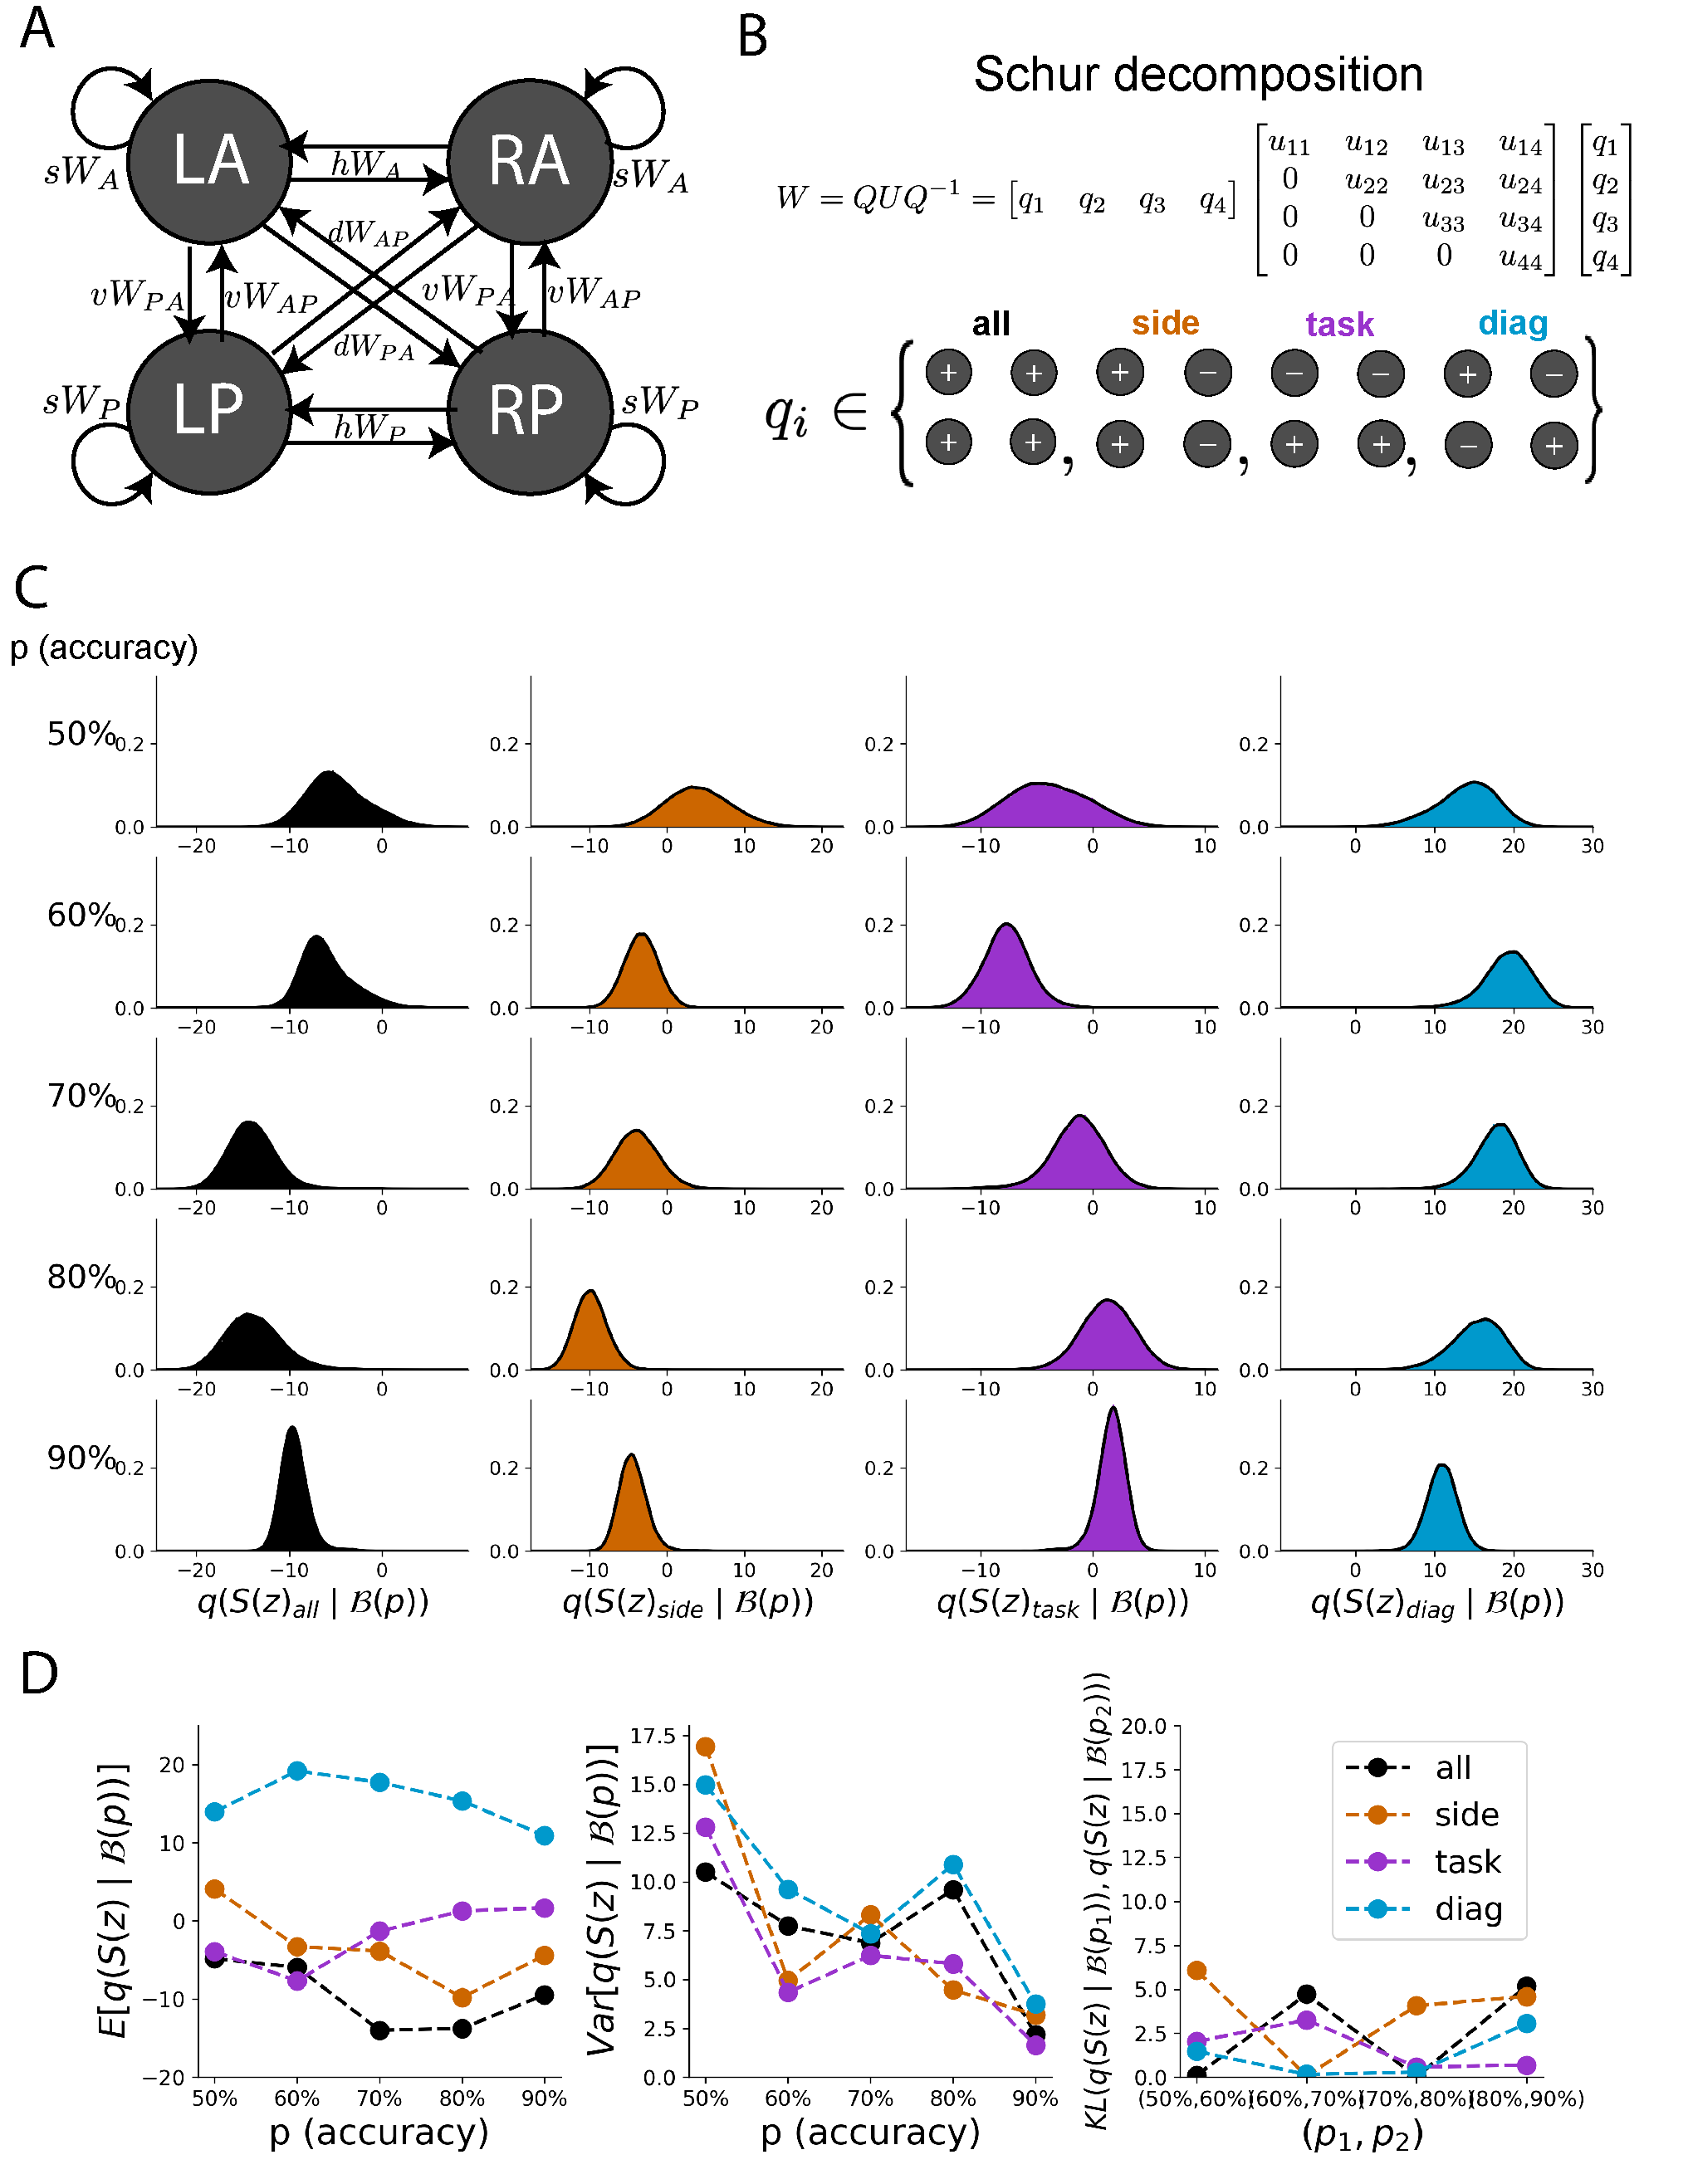
\includegraphics[scale=0.38]{images/SC_Fig.pdf}
\caption{A. Rapid task switching behavioral paradigm. In the Pro (Anti) condition indicated by an auditory cue, the rats are to respond to the same (opposite) side as the light stimulus that is provided after a delay to receive a reward. B. SC model. Neurons: LP - left pro, RP - right pro, LA - left anti, RA - right anti.  Parameters: sW - self, hW - horizontal, vW -vertical, dW - diagonal weights. C. The Schur decompostion of the weight matrix. D. The marginal EPI distributions of the Schur eigenvalues at each level of task accuracy. E. The correlation of Schur eigenvalue with task performance.}
\vspace{0.5cm}
\end{wrapfigure}
\hspace{0.4cm} In a rapid task switching experiment, rats were to respond right (R) or left (L) to the side of a light stimulus in the pro (P) task, and oppositely in the anti (A) task predicated by an auditory cue (Fig. 2A). Neural recordings exhibited two population of neurons in each hemisphere of superior colliculus (SC) that  represented both task condition and motor response: the pro/contra and anti/ipsi neurons \cite{duan2018collicular}.  Duan et al. proposed a four-population dynamical model of SC with a Pro- and Anti-population in each hemisphere, where a high output of the Pro neurons corresponds to the  contralateral response. The connectivity is parameterized by the geometry of the network (Fig. 2B).

 We ran EPI to learn distributions of SC model parameters $z = W$ consistent with various levels of rapid task switching accuracy $\mathcal{B}(p)$ for $p \in \{50\%, 60\%, 70\%, 80\%, 90\%\}$.  This gave us a broad distribution of connectivity profiles consistent with a given level of performance in the behavioral paradigm.  The Schur decomposition of $W$ has the same eigenvectors for all $W$s under this symmetric parameterization (Fig. 2C).
These consistent Schur eigenvectors have intuitive roles in processing for this task, and are accordingly named the \textit{all}, \textit{side}, \textit{task}, and \textit{diag} modes. The corresponding eigenvalues $a$ (which change with $W$) indicate degree of  amplification or supression in that mode. 

With greater accuracy, the task mode is amplified, indicating the criticality of a distributed task representation at the time of stimulus presentation, (Fig. 2D, purple).  Stepping from task-naive (50\%) to task-performing (60\%) networks, there is a suppression of the side mode (Fig. 2D, orange).  We conclude that side mode suppression allows rapid task switching, and that greater task-mode increases accuracy (Fig. 2E).  These findings motivate experimental predictions, in which the connectvity between these populations changes with accuracy such that the eigenvalues of the task mode increase  and the side mode decrease.   [1] Paninski et al. CONB, 2018. [2] Bittner et al. COSYNE, 2019. [3] Duan et al. BioRxiv, 2018.

\bibliography{Cosyne2020}
\bibliographystyle{unsrt}

\end{document}

